% This is text associated with the open textbook "Open Electromagnetics"
% See immediately below for author, date
% This work is licensed under the Creative Commons Attribution-ShareAlike 4.0 International License. (CC BY SA 4.0) 
% To view a copy of the license, visit http://creativecommons.org/licenses/by-sa/4.0/

%ORB TITLE Types of Waves  
%ORB AUTHOR 0       # S.W. Ellingson, Virginia Tech (ellingson@vt.edu)
%ORB DATE   20180807
%ORB ABSTRACT Introduction to planar, cylindrical, and spherical waves

\label{m0142_Types_of_Waves} % <-- Must match name of this file and module directory name.  Don't mess with this!

Solutions to the electromagnetic wave equations (Section~\ref{m0036_Wave_Equations_SourceFree_Lossless}) exist in a variety of forms, representing different types of waves. 
It is useful to identify three particular geometries for unguided waves. Each of these geometries is defined by the shape formed by surfaces of constant phase, which we refer to as \emph{phasefronts}.  
\index{phasefront}
(Keep in mind the analogy between electromagnetic waves and sound waves (described in Section~\ref{m0074_Fundamentals_of_Waves}), and note that sound waves also exhibit these geometries.)

A \emph{spherical wave} 
\index{waves!spherical}
has phasefronts that form concentric spheres, as shown in Figure~\ref{m0142_fSphericalPhasefront}.
Waves are well-modeled as spherical when the dimensions of the source of the wave are small relative to the scale at which the wave is observed.  
For example, the wave radiated by an antenna having dimensions of 10~cm, when observed in free space over a scale of 10~km, appears to have phasefronts that are very nearly spherical.
Note that the magnitude of the field on a phasefront of a spherical wave may vary significantly, but it is the shape of phasefronts that make it a spherical wave.
%
\begin{figure}
\begin{center}
\pdftooltip{{  % note double braces
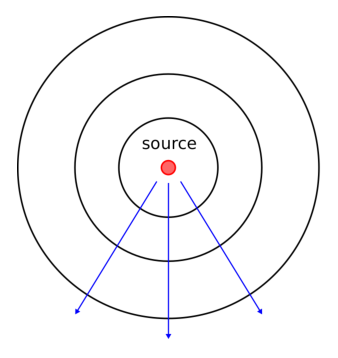
\includegraphics[width=2.5in]{modules/m0142_fSphericalPhasefront.eps}
% https://commons.wikimedia.org/wiki/File:M0142_fSphericalPhasefront.svg
}}{Three concentric circles, with a small red dot in the middle representing a source. From the source, three blue vectors extend down to the bottom left, directly below, and to the bottom right.}
\end{center} 
\centerline{\scriptsize 
\copyright~\hyperref[m0142_fSphericalPhasefront_Credit]{Y.\ Qin} 
\href{https://creativecommons.org/licenses/by/4.0/}{CC BY 4.0} 
} 
\caption{
\label{m0142_fSphericalPhasefront}
The phasefronts of a spherical wave form concentric spheres.
}
\end{figure}

A \emph{cylindrical wave} 
\index{waves!cylindrical}
exhibits phasefronts that form concentric cylinders, as shown in Figure~\ref{m0142_fCylindricalPhasefront}.
Said differently, the phasefronts of a cylindrical wave are circular in one dimension, and planar in the perpendicular direction.
A cylindrical wave is often a good description of the wave that emerges from a line-shaped source.
%
\begin{figure}
\begin{center}
\pdftooltip{{  % note double braces
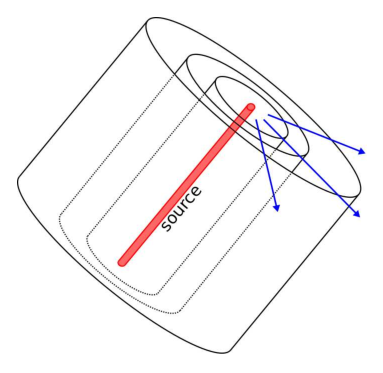
\includegraphics[width=2.5in]{modules/m0142_fCylindricalPhasefront.eps}
% https://commons.wikimedia.org/wiki/File:M0142_fCylindricalPhasefront.svg
}}{Three concentric cylinders, turned to the side so that the flat ends are pointing diagonally to the right. In the middle of the cylinders is a small red cylinder representing a source. From the source, three blue vectors extend along the face of the cylinders in the same directions as in a previous figure.}
\end{center} 
\centerline{\scriptsize 
\copyright~\hyperref[m0142_fCylindricalPhasefront_Credit]{Y.\ Qin} 
\href{https://creativecommons.org/licenses/by/4.0/}{CC BY 4.0} 
} 
\caption{
\label{m0142_fCylindricalPhasefront}
The phasefronts of a cylindrical wave form concentric cylinders.
}
\end{figure}

A \emph{plane wave} 
\index{waves!plane}
exhibits phasefronts that are planar, with planes that are parallel to each other as shown in Figure~\ref{m0142_fPlanarPhasefront}.
There are two conditions in which waves are well-modeled as plane waves.
First, some structures give rise to waves that appear to have planar phasefronts over a limited area; a good example is the wave radiated by a parabolic reflector, as shown in Figure~\ref{m0142_fPlaneWavesReflector}.
Second, all waves are well-modeled as plane waves when observed over a small region located sufficiently far from the source.
In particular, spherical waves are ``locally planar'' in the sense that they are well-modeled as planar when observed over a small portion of the spherical phasefront, as shown in Figure~\ref{m0142_fLocallyPlanar}.  
An analogy is that the Earth seems ``locally flat'' to an observer on the ground, even though it is clearly spherical to an observer in orbit.
The ``locally planar'' approximation is often employed because it is broadly applicable and simplifies analysis.
%
\begin{figure}
\begin{center}
\pdftooltip{{  % note double braces
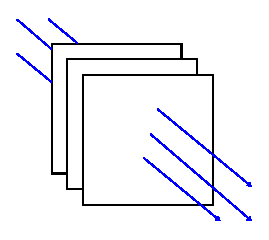
\includegraphics[width=2in]{modules/m0142_fPlanarPhasefront.eps}
% https://commons.wikimedia.org/wiki/File:M0142_fCylindricalPhasefront.svg
}}{Three square planes of the same size, laid on top of each other so that all are visible. Three equidistant blue vectors are shown behind the planes and extending from the middle of the front plane to show movement of the planes. }
\end{center} 
\centerline{\scriptsize 
\copyright~\hyperref[m0142_fPlanarPhasefront_Credit]{Y.\ Qin} 
\href{https://creativecommons.org/licenses/by/4.0/}{CC BY 4.0} 
} 
\caption{
\label{m0142_fPlanarPhasefront}
The phasefronts of a plane wave form parallel planes.
}
\end{figure}
%
\begin{figure}
\begin{center}
\pdftooltip{{  % note double braces
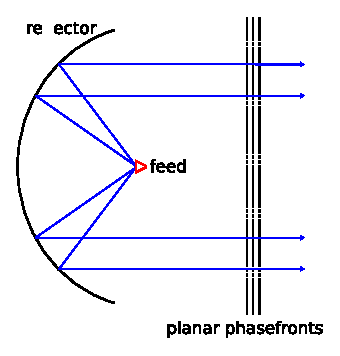
\includegraphics[width=2in]{modules/m0142_fPlaneWavesReflector.eps}
% https://commons.wikimedia.org/wiki/File:M0142_fPlaneWavesReflector.svg
}}{A parabolic reflector with open ends at slightly more than 90 degrees and less than 270 degrees to the left of three vertical dashed lines representing planar phasefronts. Between the reflector and the phasefronts is a small red triangle with the top pointed toward the phasefronts, representing feed. Four blue vectors extend from the left of the feed toward the reflector with the top two at slightly different angles and exactly mirroring the bottom two. After hitting the reflector, they follow a horizontal path right showing the direction of motion of the phasefronts.}
\end{center} 
\centerline{\scriptsize 
\copyright~\hyperref[m0142_fPlaneWavesReflector_Credit]{Y.\ Qin} 
\href{https://creativecommons.org/licenses/by/4.0/}{CC BY 4.0} 
} 
\caption{
\label{m0142_fPlaneWavesReflector}
Plane waves formed in the region in front of a parabolic reflector antenna.
}
\end{figure}
%
\begin{figure}
\begin{center}
\pdftooltip{{  % note double braces
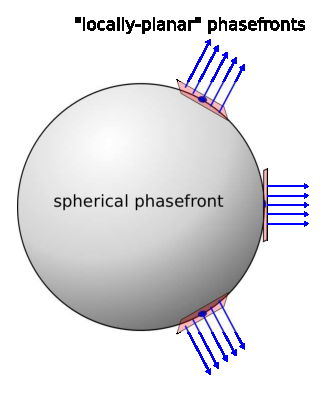
\includegraphics[width=2in]{modules/m0142_fLocallyPlanar.eps}
% https://commons.wikimedia.org/wiki/File:M0142_fLocallyPlanar.svg
}}{A three dimensional sphere, labeled "spherical phasefront". Tangent to the sphere are three red squares: one on the right, one on the upper right, and one on the lower right. From each of the red squares extends five blue vectors, pointing perpendicularly away from the sphere.}
\end{center} 
\centerline{\scriptsize 
\copyright~\hyperref[m0142_fLocallyPlanar_Credit]{Y.\ Qin} 
\href{https://creativecommons.org/licenses/by/4.0/}{CC BY 4.0} 
} 
\caption{
\label{m0142_fLocallyPlanar}
``Locally planar'' approximation of a spherical wave over a limited area.
}
\end{figure}

%ORB HIGHLIGHT
\begin{mdframed}[backgroundcolor=yellow!20,nobreak=true] 
Most waves are well-modeled as spherical, cylindrical, or plane waves.  
\end{mdframed}

%ORB HIGHLIGHT
\begin{mdframed}[backgroundcolor=yellow!20,nobreak=true] 
Plane waves (having planar phasefronts) are of particular importance due to wide applicability of the ``locally planar'' approximation. 
\end{mdframed}

